% !TEX root = ../main.tex

\section{Introduction}
\label{sec:introduction}
In this lab we get acquainted with the core concepts of computing on GPUs. We do this with some exercises in python, specifically the nNmba package that uses the Nvidia CUDA toolkit. We first look at an example that leverages the power of GPU computing and its performance is compared to that of the CPU. After we create some kernel functions and compare the time it takes to compute the result, we then compare those result.

The code repository can be found at: \\
\url{https://github.com/imstevenxyz/geavanceerde-computerarch}

\section{DFT}
\label{sec:dft}

\subsection{Kernel functions}
\label{subsec:kernel_functions}

From the given CPU based code we create two kernel functions, one that is completely parallel and one that only uses one thread.

The complete parallel function is seen in listing \ref{lst:dft_kernel_par}, here we remove one for loop from the CPU based function. To make sure that each sample gets a single thread we need to map them. For example, if we have 500 samples we enter \code{[1,500]} in the function as seen on line 1. By this we mean 1 block with 500 threads, a total of $1*500$ threads and so mapping each sample to only one thread.

\begin{lstlisting}[language=Python,caption={DFT parallel kernel},label={lst:dft_kernel_par}]
kernel_parallel[1,500](sig_sum, frequencies_real, frequencies_img)

@cuda.jit
def kernel_parallel(samples, frequencies_real, frequencies_img):
    '''Use the GPU for generating the dft. In parallel.'''

    # Calculate the thread's absolute position within the grid
    x = cuda.threadIdx.x + cuda.blockIdx.x * cuda.blockDim.x

    sample = samples[x]

    for k in range(frequencies_img.shape[0]):
        cuda.atomic.add(frequencies_real, k, ((sample * (cos(2 * pi * k * x / N)))))
        cuda.atomic.add(frequencies_img, k, ((sample * (-1* sin(2 * pi * k * x / N) ))))
\end{lstlisting}

\newpage

\subsection{Timing results}
\label{subsec:timing results}

In figure \ref{figure:function_timing} we see the timing performance of the three functions using different sample timings. To make sure we have comparable times we use the supplied \code{synchronous\_kernel\_timeit} function and always compile the kernel function beforehand. It is clear that the parallel kernel function is the best performing of the three as it stays relatively flat.
The CPU function as thought is the worst performing but if we use \code{@numba.jit} \ref{figure:jit_function_timing} we get similar timing results as the GPU parallel function.

\begin{figure}[!htb]
    \centering
    \begin{minipage}[t]{0.45\linewidth}
        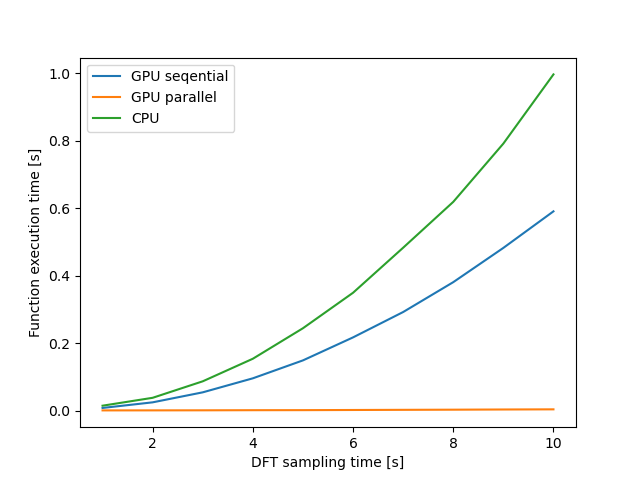
\includegraphics[width=\linewidth]{images/function_timing.png}
        \caption{Timing performance}
        \label{figure:function_timing}
    \end{minipage}
    \begin{minipage}[t]{0.45\linewidth}
        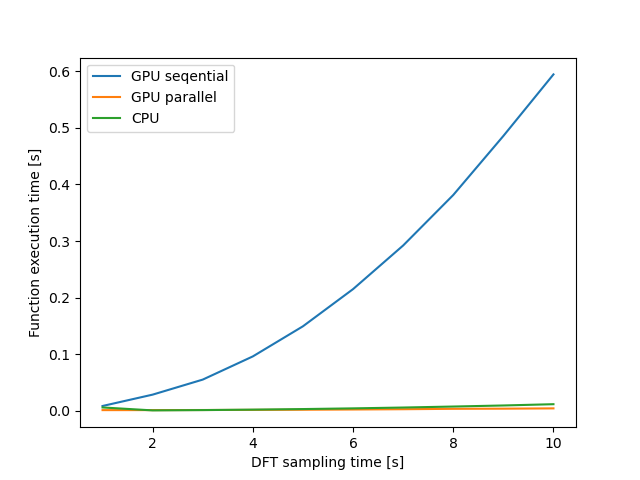
\includegraphics[width=\linewidth]{images/jit_function_timing.png}
        \caption{With @numba.jit}
        \label{figure:jit_function_timing}
    \end{minipage}
\end{figure}

\subsection{Semi parallel}
\label{subsec:semiparallel}
The function will now be partially parallel, some threads will have to loop a few times, how many times it will have to loop depends if there are fewer threads than samples. The execution time is expected to decrease as we increase the amount of threads. We perfomed this with 1 thread (full sequential) up to 500 threads (full parrallel) were we allocated always 1 more thread than before, the result of this can be seen in \ref{figure:timing_dft_S500_T500_I1.png}.
The results are not completly expected. We do see that the time decreases in steps this is because as long as 1 threads still has to do a loop the time will be longer. We also see at the beginning the time increases (peak at ~32) in this bracket more threads will increase the time, this can be with allocation of the threads takes more time. An wrong result is that the time of 500 (full parallel) is already reached at 251, this is probably an error in the code that doesnt round correctly and gives to many threads. The time on the graph are there for not accurate but the form of the graph is, (time is 1 repeat loop of).
So we can still see how much faster it will opperate when we use more threads. The biggest change is at the start where from 1 to 2 threads the time halves. But the more threads we allocate the lessen there impact on the time will be, for more it seems that 10x the amount of threads are needed to halve the time each time.


\begin{figure}
   \begin{minipage}[t]{0.45\linewidth}
        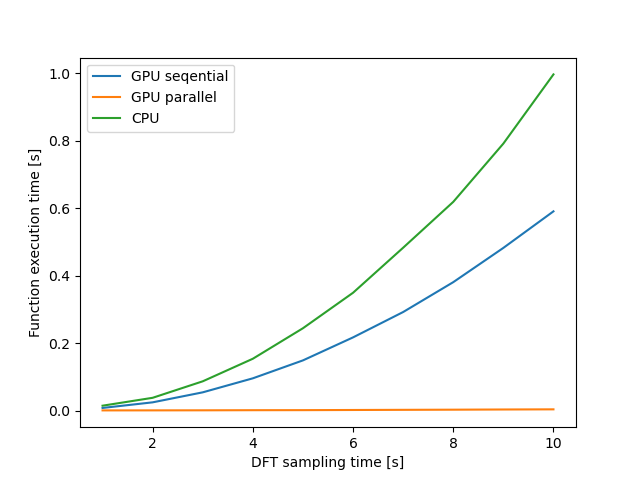
\includegraphics[width=\linewidth]{images/function_timing.png}
        \caption{Timing performance}
        \label{figure:semiparallel}
    \end{minipage}
\end{figure}

\section{Conclusion}
\label{sec:conclusion}
A CPU takes longer to execute functions than a GPU and fully parallel GPU works significantly faster. When the data gets bigger as long as you remain full paralel the time remains similair. From sequential to parralel more threads are better for execution time but there are diminishing returns the more threads we use.

